\documentclass[10pt]{beamer}

% Theme Setup
\usetheme{Boadilla}
\usecolortheme{default}

% Accenture Branding Colors
\definecolor{accenturepurple}{HTML}{A100FF}    % Accenture Purple
\definecolor{accentureblack}{HTML}{111111}     % Deep Black
\definecolor{accenturegray}{HTML}{F4F4F4}      % Light Accent Gray
\definecolor{accenturedarkgray}{HTML}{3A3A3A}  % Dark Gray

% Apply Color Palette to Beamer Elements
\setbeamercolor{structure}{fg=accenturepurple}
\setbeamercolor{titlelike}{bg=accentureblack,fg=white}
\setbeamercolor{author}{fg=accenturedarkgray}
\setbeamercolor{date}{fg=accenturedarkgray}
\setbeamercolor{institute}{fg=accenturedarkgray}
\setbeamercolor{frametitle}{bg=accentureblack,fg=white}
\setbeamercolor{block title}{bg=accenturepurple,fg=white}
\setbeamercolor{block body}{bg=accenturegray,fg=accentureblack}

% Package Imports
\usepackage[utf8]{inputenc}
\usepackage{booktabs}
\usepackage{array}
\usepackage{tikz}
\usetikzlibrary{shapes.geometric, arrows.meta, positioning, shadow, calc, fit}

\newcolumntype{L}[1]{>{\raggedright\let\newline\\\arraybackslash\hspace{0pt}}m{#1}}
\newcolumntype{C}[1]{>{\centering\let\newline\\\arraybackslash\hspace{0pt}}m{#1}}

% Presentation Metadata
\title[Personal AI Assistant]{PERSONAL AI ASSISTANT}
\subtitle{Architecture, Data Ingestion, and Multi-Agent Design of a Personal AI Workspace Productivity Assistant}
\author[Radesh \& Sai Sameer]{Radesh and Sai Sameer}
\institute[Accenture]{AI Research and Systems Engineering \\ AEH Interns, Accenture}
\date[July 2026]{July 2026}

\begin{document}

% Slide 1: Title Slide
\begin{frame}
  \titlepage
\end{frame}

% Slide 2: Background & Problem Statement
\begin{frame}{Introduction: The Problem}
  \begin{itemize}
    \item \textbf{Fragmentation:} Knowledge workers navigate multiple communication silos daily (Gmail, Google Calendar, WhatsApp, Discord).
    \item \textbf{Cognitive Fatigue:} Constantly context-switching to search for files, conversation histories, and agendas reduces work output.
    \item \textbf{Lost Insights:} Key commitments, decisions, and action lists are easily lost in transient instant messaging threads.
    \item \textbf{Manual overhead:} Manually recording meeting minutes and transcribing audio files is extremely time-consuming.
  \end{itemize}
  \vfill
  \begin{block}{The Solution}
    A central, conversational AI assistant serving as an omnipresent workspace cognitive extension.
  \end{block}
\end{frame}

% Slide 3: Project Scope & Objectives
\begin{frame}{Project Objectives}
  \begin{itemize}
    \item \textbf{Data Consolidation:} Sync Gmail, Google Calendar, WhatsApp logs, and Fireflies meeting records into a single knowledge base.
    \item \textbf{Conversational Interfaces:} Access and query workspace memory directly through Discord chats and WhatsApp messages.
    \item \textbf{Relational-Vector Memory:} Use a hybrid relational-vector store (**GBrain**) to query records semantically and through full-text keywords.
    \item \textbf{Automated Summaries:} Compile daily review digests, generate meeting prep summaries, and trigger automated alerts.
  \end{itemize}
\end{frame}

% Slide 4: Architectural Tiers
\begin{frame}{System Tier Architecture}
  The assistant is structured into three main layers:
  \begin{enumerate}
    \item \textbf{Interface Gateway Tier}
      \begin{itemize}
        \item Captures messages, audio recordings, and commands via Discord and WhatsApp.
      \end{itemize}
    \item \textbf{Orchestration \& Agent Tier}
      \begin{itemize}
        \item Uses the \textbf{GStack} framework to parse intents and route them to target specialist AI agents.
      \end{itemize}
    \item \textbf{Data \& Memory Layer}
      \begin{itemize}
        \item Manages vector indexing, database storage (**GBrain**), and LLM generation (**Gemini**).
      \end{itemize}
  \end{enumerate}
\end{frame}

% Slide 5: System Architecture Diagram
\begin{frame}{End-to-End System Architecture}
  \centering
  \begin{tikzpicture}[
      scale=0.62, every node/.style={transform shape},
      box/.style={draw=structure, fill=accenturegray, rectangle, rounded corners=3pt, minimum width=3.4cm, minimum height=0.7cm, align=center, font=\scriptsize\bfseries, line width=1pt},
      agent/.style={draw=accenturepurple, fill=accenturepurple!15, rectangle, rounded corners=4pt, minimum width=1.8cm, minimum height=0.65cm, align=center, font=\scriptsize\bfseries, line width=1pt},
      arrow/.style={-Latex, line width=1pt, draw=accentureblack},
      bidir/.style={Latex-Latex, line width=1pt, draw=structure}
  ]
      % Nodes
      \node (user_channels) [box] at (0, 0) {User Communication Channels \\ (Discord / WhatsApp / Telegram / Audio)};
      \node (openclaw_gateway) [box] at (0, -1.2) {OpenClaw Gateway Service \\ (Agent Runtime Gateway)};
      \node (discord_bot) [box] at (-2.8, -2.6) {Discord Bot \\ \texttt{discord-bot.mjs}};
      \node (wa_webhook) [box] at (2.8, -2.6) {WhatsApp Webhook \\ \texttt{whatsapp-webhook.mjs}};
      \node (orchestrator) [box] at (0, -4.0) {GStack Orchestrator \\ \texttt{agents/orchestrator.mjs}};
      
      % 5 Agents
      \node (email_agent) [agent] at (-4.4, -5.4) {Email Agent};
      \node (memory_agent) [agent] at (-2.2, -5.4) {Memory Agent};
      \node (calendar_agent) [agent] at (0, -5.4) {Calendar Agent};
      \node (whatsapp_agent) [agent] at (2.2, -5.4) {WhatsApp Agent};
      \node (meetings_agent) [agent] at (4.4, -5.4) {Meetings Agent};
      
      % Bottom Layer
      \node (gemini_engine) [box] at (4.4, -8.3) {Gemini LLM Engine \\ (intent parsing, summaries)};

      % Manual Cylinder
      \draw[draw=structure, fill=accenturegray, line width=1pt] (0, -9.1) ellipse (1.4cm and 0.3cm);
      \fill[fill=accenturegray] (-1.4, -9.1) rectangle (1.4, -7.6);
      \draw[draw=structure, line width=1pt] (-1.4, -9.1) -- (-1.4, -7.6);
      \draw[draw=structure, line width=1pt] (1.4, -9.1) -- (1.4, -7.6);
      \draw[draw=structure, fill=accenturepurple!20, line width=1pt] (0, -7.6) ellipse (1.4cm and 0.3cm);
      \node[align=center, font=\tiny\bfseries, text=accentureblack] at (0, -8.3) {GBrain Database \\ (PGLite / Postgres)};

      \coordinate (db_top) at (0, -7.3);
      \coordinate (db_left) at (-1.4, -8.3);
      \coordinate (db_right) at (1.4, -8.3);

      % Arrows
      \draw [arrow] (user_channels) -- (openclaw_gateway);
      \draw [arrow] (openclaw_gateway.south) -| (discord_bot.north);
      \draw [arrow] (openclaw_gateway.south) -| (wa_webhook.north);
      \draw [arrow] (discord_bot.south) -- (orchestrator.north-west);
      \draw [arrow] (wa_webhook.south) -- (orchestrator.north-east);
      \draw [arrow] (orchestrator) -- (email_agent.north);
      \draw [arrow] (orchestrator) -- (memory_agent.north);
      \draw [arrow] (orchestrator) -- (calendar_agent.north);
      \draw [arrow] (orchestrator) -- (whatsapp_agent.north);
      \draw [arrow] (orchestrator) -- (meetings_agent.north);
      \draw [arrow] (email_agent.south) |- ($(db_left) + (0, -0.3)$);
      \draw [arrow] (memory_agent.south) |- ($(db_left) + (0, 0.3)$);
      \draw [arrow] (calendar_agent.south) -- (db_top);
      \draw [arrow] (whatsapp_agent.south) |- ($(db_right) + (0, 0.3)$);
      \draw [arrow] (meetings_agent.south) -- (gemini_engine.north);
      \draw [bidir] (db_right) -- (gemini_engine.west);
  \end{tikzpicture}
\end{frame}

% Slide 6: Interface Gateway Tier Details
\begin{frame}{Interface Gateways: Discord \& WhatsApp}
  \begin{block}{Discord Client (\texttt{discord-bot.mjs})}
    \begin{itemize}
      \item Powered by \texttt{discord.js} with Guild Message and Content Intents.
      \item Handles user commands, file attachment uploads, and short voice notes.
      \item Enforces a 2000-character split mechanism to handle long response formats.
    \end{itemize}
  \end{block}
  \begin{block}{WhatsApp Webhook Gateway (\texttt{whatsapp-webhook.mjs})}
    \begin{itemize}
      \item Fast HTTP endpoint integration with Meta Cloud API.
      \item Implements subscriber token handshakes.
      \item Parses message structures, matches user profiles, and delivers outbound notifications.
    \end{itemize}
  \end{block}
\end{frame}

% Slide 7: Orchestration Tier Details
\begin{frame}{Agent Orchestration: GStack}
  \begin{itemize}
    \item Bypasses complex regex commands using Large Language Models as routers.
    \item \textbf{Core Logic} (\texttt{agents/orchestrator.mjs}):
      \begin{itemize}
        \item Submits user prompts to Google Gemini.
        \item Classifies requests into structured, parameterized intents.
        \item Routes tasks to the correct specialized agent.
      \end{itemize}
    \item **Context Preservation:** Keeps track of confirmation prompts (e.g. preparing and reviewing meeting summaries).
  \end{itemize}
  \vfill
  \begin{block}{Gemini Integration}
    Uses Gemini 1.5 Flash and Gemini 2.5 Flash for high translation speeds and a 1-million-token context window.
  \end{block}
\end{frame}

% Slide 8: Intent Classification Matrix
\begin{frame}{GStack Intent Mapping Matrix}
  \centering
  \scriptsize
  \begin{tabular}{L{3.0cm} L{2.2cm} L{6.0cm}}
    \toprule
    \textbf{Parsed Intent} & \textbf{Specialist Agent} & \textbf{Operational Function} \\
    \midrule
    \texttt{search\_emails} & Email Agent & Context search over email records in GBrain. \\
    \texttt{summarize\_emails} & Email Agent & Generates daily email summaries. \\
    \texttt{important\_emails} & Email Agent & Ranks emails by priority metrics. \\
    \texttt{action\_items} & Email Agent & Extracts user commitments and deadlines. \\
    \texttt{daily\_report} & Summary Agent & Consolidates status, calendars, and tasks. \\
    \texttt{meeting\_prep} & Meetings Agent & Gathers relevant summaries for upcoming events. \\
    \texttt{search\_whatsapp} & WhatsApp Agent & Searches WhatsApp messaging archives. \\
    \texttt{general\_query} & Memory Agent & Triggers database-wide fallback searches. \\
    \bottomrule
  \end{tabular}
\end{frame}

% Slide 9: Specialist AI Agents (Tier 1)
\begin{frame}{Specialist AI Agents: Email, Memory \& Calendar}
  \begin{itemize}
    \item \textbf{Email Agent (\texttt{agents/email-agent.mjs}):}
      \begin{itemize}
        \item Runs semantic searches over historical emails.
        \item Scores and sorts emails based on priority keywords.
        \item Extracts user-specific deadlines and tasks.
      \end{itemize}
    \vspace{0.3cm}
    \item \textbf{Memory Agent (\texttt{agents/memory-agent.mjs}):}
      \begin{itemize}
        \item Coordinates general information retrieval.
        \item Runs database-wide queries to retrieve relevant context.
      \end{itemize}
    \vspace{0.3cm}
    \item \textbf{Calendar Agent (\texttt{agents/calendar-agent.mjs}):}
      \begin{itemize}
        \item Interfaces with the Google Calendar API helper.
        \item Fetches event descriptions, organizer contacts, and meeting links.
      \end{itemize}
  \end{itemize}
\end{frame}

% Slide 10: Specialist AI Agents (Tier 2)
\begin{frame}{Specialist AI Agents: WhatsApp, Meetings \& Summary}
  \begin{itemize}
    \item \textbf{WhatsApp Agent (\texttt{agents/whatsapp-agent.mjs}):}
      \begin{itemize}
        \item Indexes user chat threads into the vector store.
        \item Generates context-aware replies for Meta Business API delivery.
      \end{itemize}
    \vspace{0.3cm}
    \item \textbf{Meetings Agent (\texttt{agents/meetings-agent.mjs}):}
      \begin{itemize}
        \item Handles transcripts, action items, and decisions from audio files.
        \item Syncs external summaries using Fireflies.ai GraphQL clients.
      \end{itemize}
    \vspace{0.3cm}
    \item \textbf{Summary Agent (\texttt{agents/summary-agent.mjs}):}
      \begin{itemize}
        \item Compiles the morning digest review (agendas, pending tasks, emails).
      \end{itemize}
  \end{itemize}
\end{frame}

% Slide 11: Data & Memory Layer (GBrain)
\begin{frame}{Knowledge Engine: GBrain}
  \begin{itemize}
    \item \textbf{Hybrid Engine:} Combines relational SQL properties with pgvector embedding properties.
    \item **Semantic Vector Matching:** Converts text queries to 1536-dimension vector arrays using Gemini embeddings, measuring similarity distance against documents.
    \item **Local Footprint:** File-backed WASM PostgreSQL runtime (PGLite) storing data in \texttt{\textasciitilde{}/.gbrain/brain.pglite} within WSL.
    \item **Production Portability:** Connects to native Docker/cloud PostgreSQL servers without requiring codebase alterations.
  \end{itemize}
  \vfill
  \begin{block}{Fallback Capability}
    If vector models are unavailable, GBrain automatically falls back to full-text keyword indexing (FTS).
  \end{block}
\end{frame}

% Slide 12: Database Schema & Document Models
\begin{frame}{Relational Schema \& Document Templates}
  \begin{block}{Relational Schema}
    \begin{itemize}
      \item \texttt{documents}: Stores the raw text, unique slug, and meta variables.
      \item \texttt{document\_embeddings}: Stores vector values mapped to the main document IDs.
    \end{itemize}
  \end{block}
  \begin{block}{Standard Document Templates}
    Saved as structured Markdown templates to help the LLM parser locate metadata:
    \begin{itemize}
      \item \textbf{Emails:} \texttt{\# Email: [Subject] \\ From: [Sender] \\ Body...}
      \item \textbf{Events:} \texttt{\# Calendar Event: [Title] \\ Start: [Time] \\ Link...}
      \item \textbf{Meetings:} \texttt{\# Meeting: [Title] \\ Summary... \\ Action Items...}
    \end{itemize}
  \end{block}
\end{frame}

% Slide 13: Ingestion Pipeline Workflow
\begin{frame}{Gmail & Calendar Ingestion Pipeline}
  \begin{itemize}
    \item Running as a WSL background cron task (every 30 minutes).
    \item Uses Google OAuth 2.0 (`token.json`) for authentication.
    \item \textbf{Email Deduplication:} Map incoming message IDs to unique slugs (\texttt{email-[id]}) to avoid record duplication.
    \item \textbf{Calendar Tracking:} Queries Google Calendar events for the next 48 hours.
    \item \textbf{Alert Triggering:} Evaluates start times. Pushes meeting alert notifications to Discord channels 60 minutes before meetings begin.
  \end{itemize}
\end{frame}

% Slide 14: Ingestion Pipeline Sequence
\begin{frame}{Ingestion Pipeline Flow}
  \centering
  \begin{tikzpicture}[
      scale=0.5, every node/.style={transform shape},
      node distance=1.2cm,
      lifeline/.style={draw=gray, dashed, line width=1pt},
      entity/.style={draw=structure, fill=accenturegray, rectangle, rounded corners=3pt, minimum width=2.0cm, minimum height=0.7cm, align=center, font=\scriptsize\bfseries},
      msg/.style={-Latex, line width=0.8pt, font=\tiny, align=center},
      ret/.style={-Latex, dashed, line width=0.8pt, font=\tiny, align=center},
      self/.style={-Latex, line width=0.8pt, font=\tiny, align=center}
  ]
      \def\xinterval{0} \def\xpipeline{2.2} \def\xgmail{4.8} \def\xgbrain{7.8} \def\xcalendar{10.6} \def\xdiscord{13.0} \def\xdata{15.4}

      \node (l_int) [entity] at (\xinterval, 0.5) {setInterval};
      \node (l_pip) [entity] at (\xpipeline, 0.5) {ingestion};
      \node (l_gma) [entity] at (\xgmail, 0.5) {Gmail API};
      \node (l_gbr) [entity] at (\xgbrain, 0.5) {GBrain};
      \node (l_cal) [entity] at (\xcalendar, 0.5) {Calendar};
      \node (l_dis) [entity] at (\xdiscord, 0.5) {Discord};
      \node (l_dat) [entity] at (\xdata, 0.5) {data/};

      \draw [lifeline] (\xinterval, 0) -- (\xinterval, -9.5);
      \draw [lifeline] (\xpipeline, 0) -- (\xpipeline, -9.5);
      \draw [lifeline] (\xgmail, 0) -- (\xgmail, -9.5);
      \draw [lifeline] (\xgbrain, 0) -- (\xgbrain, -9.5);
      \draw [lifeline] (\xcalendar, 0) -- (\xcalendar, -9.5);
      \draw [lifeline] (\xdiscord, 0) -- (\xdiscord, -9.5);
      \draw [lifeline] (\xdata, 0) -- (\xdata, -9.5);

      \draw [msg] (\xinterval, -0.6) -- node[above] {Trigger} (\xpipeline, -0.6);
      \draw [msg] (\xpipeline, -1.2) -- node[above] {Fetch emails} (\xgmail, -1.2);
      \draw [ret] (\xgmail, -1.8) -- node[above] {Email bodies} (\xpipeline, -1.8);
      
      \draw [msg] (\xpipeline, -2.6) -- node[above] {\texttt{documentExists}?} (\xgbrain, -2.6);
      \draw [msg] (\xpipeline, -3.4) -- node[above] {\texttt{storeDocument}} (\xgbrain, -3.4);
      \draw [msg] (\xpipeline, -4.2) -- node[above] {Save JSON backup} (\xdata, -4.2);

      \draw [msg] (\xpipeline, -5.2) -- node[above] {Fetch agenda} (\xcalendar, -5.2);
      \draw [ret] (\xcalendar, -5.8) -- node[above] {Calendar events} (\xpipeline, -5.8);
      \draw [msg] (\xpipeline, -6.6) -- node[above] {\texttt{storeCalendarEvent}} (\xgbrain, -6.6);

      \draw [msg] (\xpipeline, -7.6) -- node[above] {Send ``Meeting Alert''} (\xdiscord, -7.6);
      \draw [self] (\xpipeline, -8.6) .. controls (\xpipeline+0.7, -8.4) and (\xpipeline+0.7, -8.8) .. node[right] {Mark alert sent} (\xpipeline, -8.6);
  \end{tikzpicture}
\end{frame}

% Slide 15: User Query Sequence Flow
\begin{frame}{Conversational Query Sequence}
  \centering
  \begin{tikzpicture}[
      scale=0.52, every node/.style={transform shape},
      node distance=1.4cm,
      lifeline/.style={draw=gray, dashed, line width=1pt},
      entity/.style={draw=structure, fill=accenturegray, rectangle, rounded corners=3pt, minimum width=2.0cm, minimum height=0.7cm, align=center, font=\scriptsize\bfseries},
      msg/.style={-Latex, line width=0.8pt, font=\tiny, align=center},
      ret/.style={-Latex, dashed, line width=0.8pt, font=\tiny, align=center},
      self/.style={-Latex, line width=0.8pt, font=\tiny, align=center}
  ]
      \def\xuser{0} \def\xbot{2.4} \def\xorch{5.0} \def\xgemini{8.2} \def\xagent{11.2} \def\xgbrain{14.2}

      \node (l_usr) [entity] at (\xuser, 0.5) {User};
      \node (l_bot) [entity] at (\xbot, 0.5) {Bot / Webhook};
      \node (l_orc) [entity] at (\xorch, 0.5) {Orchestrator};
      \node (l_gem) [entity] at (\xgemini, 0.5) {Gemini};
      \node (l_age) [entity] at (\xagent, 0.5) {Special Agent};
      \node (l_gbr) [entity] at (\xgbrain, 0.5) {GBrain};

      \draw [lifeline] (\xuser, 0) -- (\xuser, -8.5);
      \draw [lifeline] (\xbot, 0) -- (\xbot, -8.5);
      \draw [lifeline] (\xorch, 0) -- (\xorch, -8.5);
      \draw [lifeline] (\xgemini, 0) -- (\xgemini, -8.5);
      \draw [lifeline] (\xagent, 0) -- (\xagent, -8.5);
      \draw [lifeline] (\xgbrain, 0) -- (\xgbrain, -8.5);

      \draw [msg] (\xuser, -0.8) -- node[above] {``Show emails from John''} (\xbot, -0.8);
      \draw [msg] (\xbot, -1.6) -- node[above] {\texttt{processCommand}} (\xorch, -1.6);
      
      \draw [msg] (\xorch, -2.6) -- node[above] {\texttt{parseIntent}} (\xgemini, -2.6);
      \draw [ret] (\xgemini, -3.4) -- node[above] {\{intent: search\_emails, sender: John\}} (\xorch, -3.4);

      \draw [msg] (\xorch, -4.4) -- node[above] {\texttt{searchEmails("John")}} (\xagent, -4.4);
      \draw [msg] (\xagent, -5.2) -- node[above] {\texttt{queryGBrain("John")}} (\xgbrain, -5.2);
      \draw [ret] (\xgbrain, -6.0) -- node[above] {Raw text records} (\xagent, -6.0);

      \draw [self] (\xagent, -6.8) .. controls (\xagent+0.7, -6.6) and (\xagent+0.7, -7.0) .. node[right] {Filter and format} (\xagent, -6.8);
      \draw [ret] (\xagent, -7.4) -- node[above] {Formatted list} (\xorch, -7.4);
      \draw [ret] (\xorch, -8.0) -- node[above] {Reply response} (\xbot, -8.0);
  \end{tikzpicture}
\end{frame}

% Slide 16: Meeting Recording Ingestion Sequence
\begin{frame}{Audio & Meeting Processing Sequence}
  \centering
  \begin{tikzpicture}[
      scale=0.52, every node/.style={transform shape},
      node distance=1.4cm,
      lifeline/.style={draw=gray, dashed, line width=1pt},
      entity/.style={draw=structure, fill=accenturegray, rectangle, rounded corners=3pt, minimum width=2.0cm, minimum height=0.7cm, align=center, font=\scriptsize\bfseries},
      msg/.style={-Latex, line width=0.8pt, font=\tiny, align=center},
      ret/.style={-Latex, dashed, line width=0.8pt, font=\tiny, align=center},
      self/.style={-Latex, line width=0.8pt, font=\tiny, align=center}
  ]
      \def\xuser{0} \def\xdiscord{2.8} \def\xvoice{5.6} \def\xtrans{8.6} \def\xsum{11.8} \def\xgbr{14.8}

      \node (l_usr) [entity] at (\xuser, 0.5) {User};
      \node (l_dis) [entity] at (\xdiscord, 0.5) {Discord Bot};
      \node (l_voi) [entity] at (\xvoice, 0.5) {Voice Handler};
      \node (l_tra) [entity] at (\xtrans, 0.5) {Transcriber};
      \node (l_sum) [entity] at (\xsum, 0.5) {Summarizer};
      \node (l_gbr) [entity] at (\xgbr, 0.5) {GBrain};

      \draw [lifeline] (\xuser, 0) -- (\xuser, -8.5);
      \draw [lifeline] (\xdiscord, 0) -- (\xdiscord, -8.5);
      \draw [lifeline] (\xvoice, 0) -- (\xvoice, -8.5);
      \draw [lifeline] (\xtrans, 0) -- (\xtrans, -8.5);
      \draw [lifeline] (\xsum, 0) -- (\xsum, -8.5);
      \draw [lifeline] (\xgbr, 0) -- (\xgbr, -8.5);

      \draw [msg] (\xuser, -0.8) -- node[above] {Upload audio file} (\xdiscord, -0.8);
      \draw [msg] (\xdiscord, -1.6) -- node[above] {\texttt{downloadAttachment}} (\xvoice, -1.6);
      \draw [ret] (\xvoice, -2.4) -- node[above] {Buffer file} (\xdiscord, -2.4);

      \draw [msg] (\xdiscord, -3.2) -- node[above] {\texttt{transcribeBuffer}} (\xtrans, -3.2);
      \draw [ret] (\xtrans, -4.0) -- node[above] {Transcript text} (\xdiscord, -4.0);

      \draw [msg] (\xdiscord, -4.8) -- node[above] {\texttt{analyzeMeeting}} (\xsum, -4.8);
      \draw [ret] (\xsum, -5.6) -- node[above] {Summary \& Action Items} (\xdiscord, -5.6);

      \draw [msg] (\xdiscord, -6.6) -- node[above] {\texttt{storeDocument}} (\gbr, -6.6);
      \draw [ret] (\xdiscord, -7.6) -- node[above] {Processing confirmation} (\xuser, -7.6);
  \end{tikzpicture}
\end{frame}

% Slide 17: User Chat Interfaces (Discord Gateway)
\begin{frame}{Interactive Gateways: Discord Bot In Action}
  \begin{columns}
    \begin{column}{0.5\textwidth}
      \textbf{Smart Email Digests}
      \begin{itemize}
        \item Automatic daily sync and priority categorization of incoming workspace mail.
        \item Classifies critical items requiring action (e.g., security alerts, important calls).
        \item Preserves context tags and provides sender details.
      \end{itemize}
    \end{column}
    \begin{column}{0.5\textwidth}
      \centering
      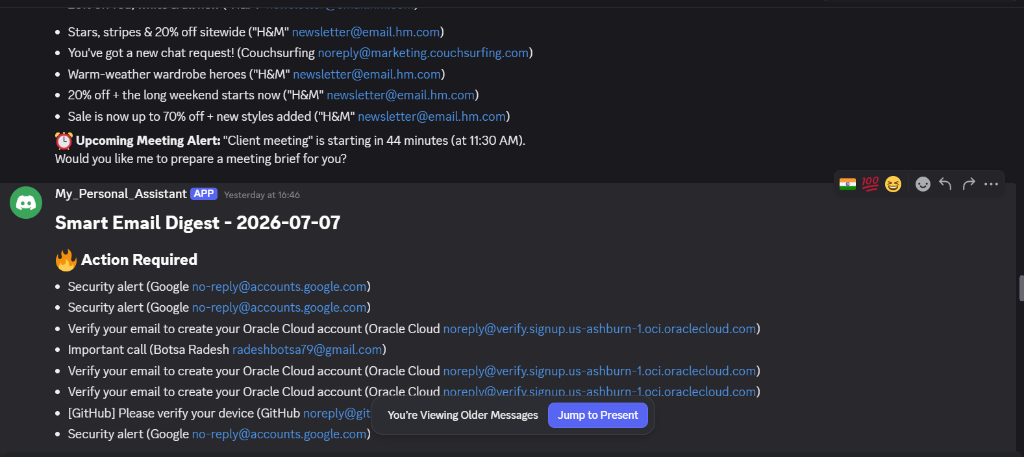
\includegraphics[width=0.95\textwidth]{images/media__1783498591044.png}
    \end{column}
  \end{columns}
\end{frame}

% Slide 18: Meeting Transcription Gateway (Discord Bot)
\begin{frame}{Interactive Gateways: Meeting Ingestion}
  \begin{columns}
    \begin{column}{0.5\textwidth}
      \textbf{Decisions & Action Items}
      \begin{itemize}
        \item Automatically indexes meeting metadata (Date, Duration, Platform, Attendees).
        \item Synthesizes meeting summary transcripts.
        \item Extracts clear ownership parameters for action items and logs them.
      \end{itemize}
    \end{column}
    \begin{column}{0.5\textwidth}
      \centering
      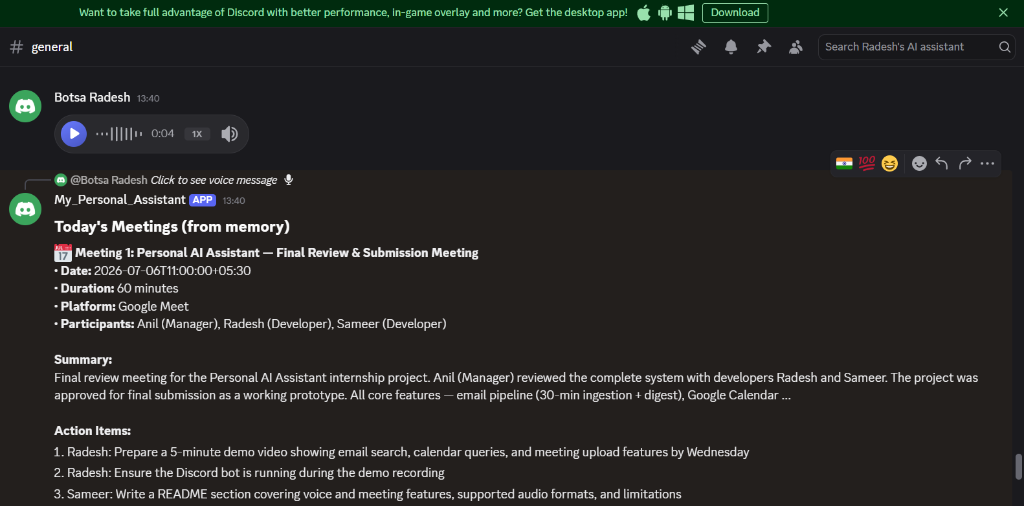
\includegraphics[width=0.95\textwidth]{images/media__1783498285665.png}
    \end{column}
  \end{columns}
\end{frame}

% Slide 19: Mobile Gateway (WhatsApp Channel)
\begin{frame}{Interactive Gateways: WhatsApp Interface}
  \begin{columns}
    \begin{column}{0.5\textwidth}
      \textbf{Omnipresent Mobile Hub}
      \begin{itemize}
        \item Delivers Daily Productivity Digests directly to WhatsApp chat interfaces.
        \item Consolidates upcoming agendas, email alerts, and priority checklists.
        \item Supports interactive query flows.
      \end{itemize}
    \end{column}
    \begin{column}{0.5\textwidth}
      \centering
      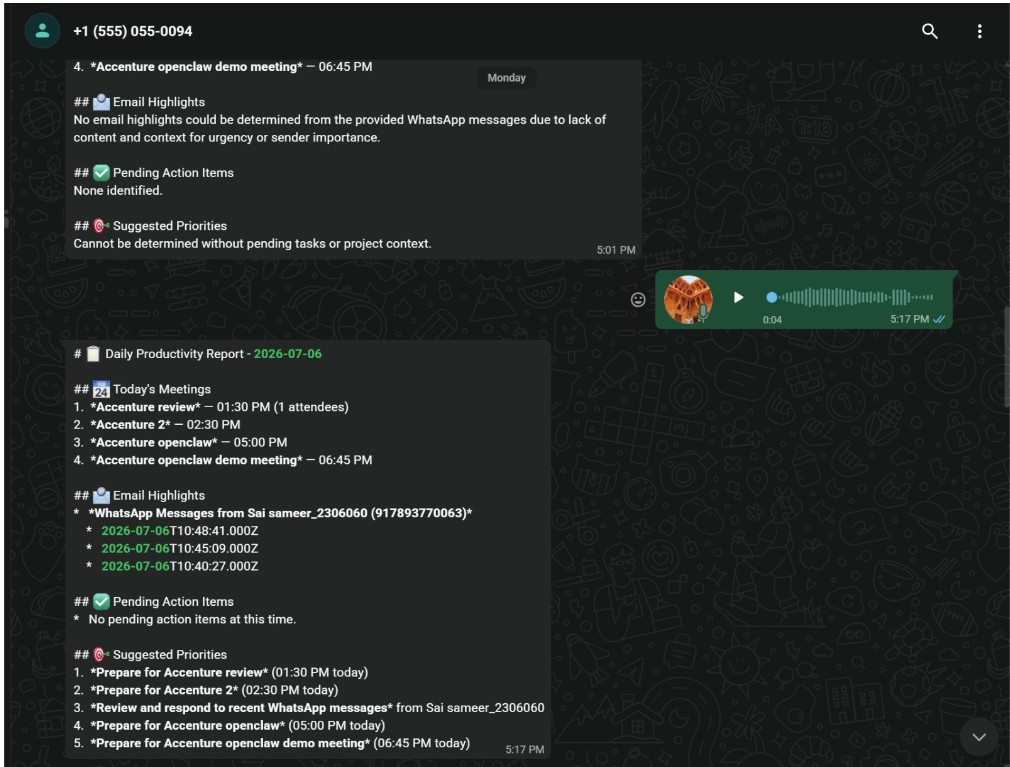
\includegraphics[width=0.85\textwidth]{images/media__1783498061253.png}
    \end{column}
  \end{columns}
\end{frame}

% Slide 20: Mobile Gateway: WhatsApp Inquiries
\begin{frame}{Interactive Gateways: Conversational Inquiries}
  \begin{columns}
    \begin{column}{0.5\textwidth}
      \textbf{Context-Aware Answers}
      \begin{itemize}
        \item Supports natural language inquiries on mobile.
        \item Users can ask: \textit{"give transcript for morning meeting"} or \textit{"meetings in next 12 hours"}.
        \item Directly queries local database memory to extract facts.
      \end{itemize}
    \end{column}
    \begin{column}{0.5\textwidth}
      \centering
      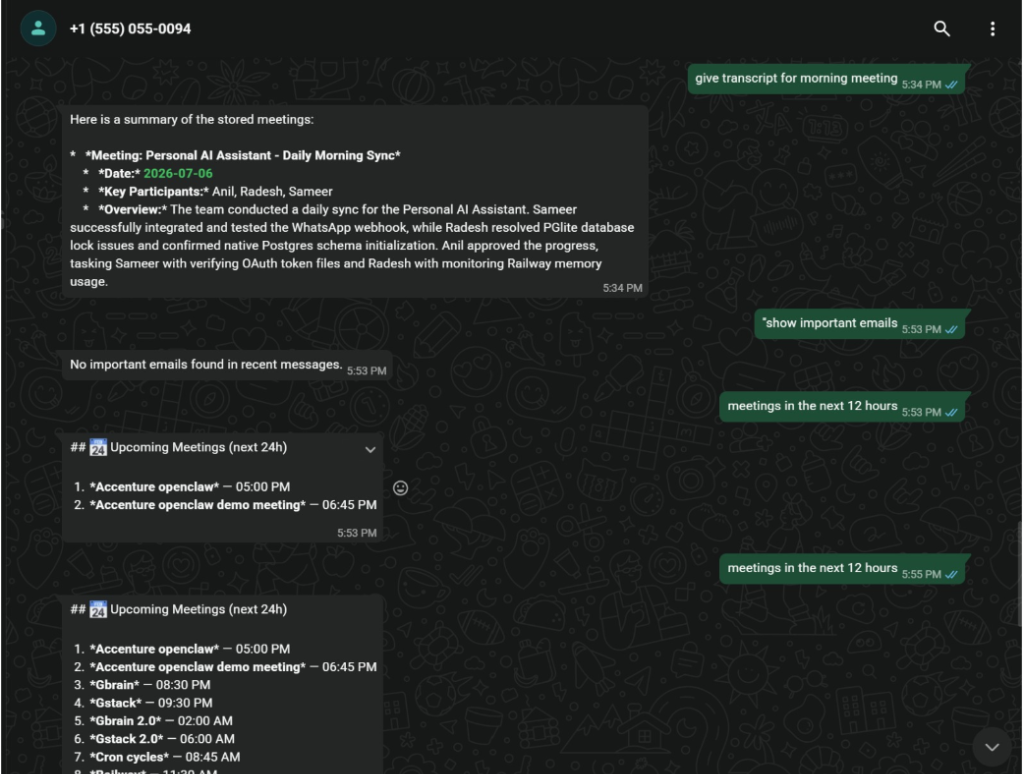
\includegraphics[width=0.85\textwidth]{images/media__1783498323059.png}
    \end{column}
  \end{columns}
\end{frame}

% Slide 21: Mobile Gateway: Telegram Bot
\begin{frame}{Interactive Gateways: Telegram Bot}
  \begin{columns}
    \begin{column}{0.5\textwidth}
      \textbf{Telegram Bot Gateway}
      \begin{itemize}
        \item Connects securely to the OpenClaw gateway using bot tokens.
        \item Restricts workspace access strictly to permitted users (via \texttt{allowedUsers}).
        \item Allows users to query emails, calendars, meeting summaries, and action lists directly.
      \end{itemize}
    \end{column}
    \begin{column}{0.5\textwidth}
      \centering
      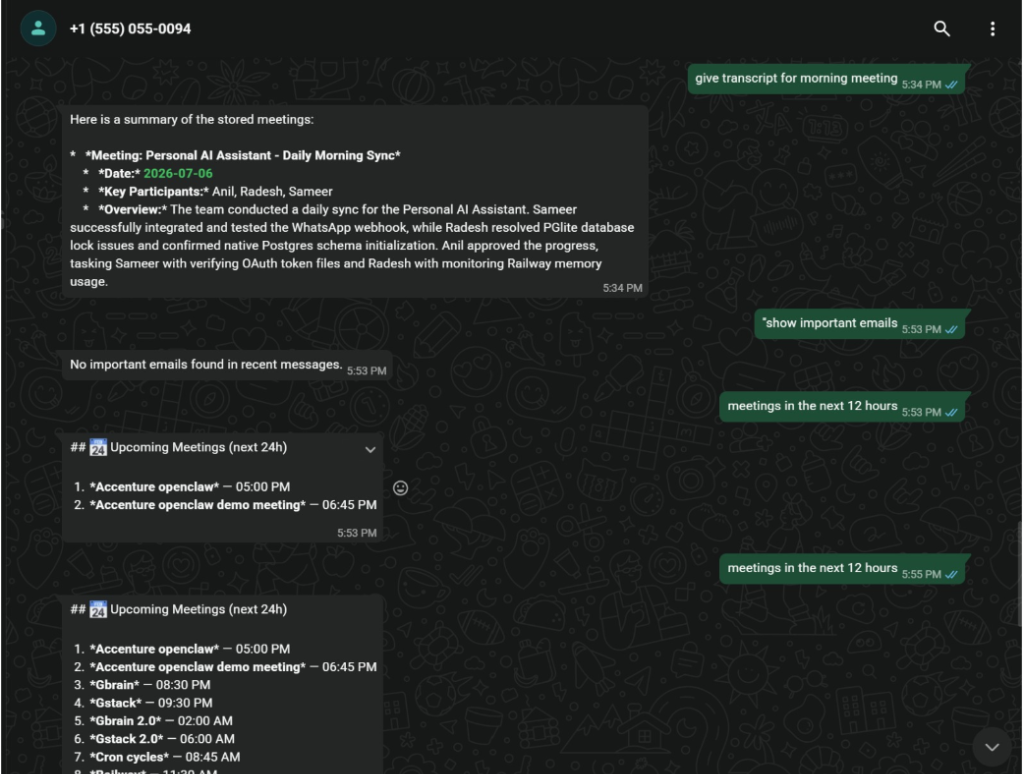
\includegraphics[width=0.85\textwidth]{images/telegram_reply.png}
    \end{column}
  \end{columns}
\end{frame}

% Slide 20: Fireflies.ai Integration
\begin{frame}{GraphQL Integrations: Fireflies.ai}
  \begin{itemize}
    \item \textbf{Target Integration:} Synchronizes transcripts directly from Fireflies cloud environments via the GraphQL API interface.
    \item \textbf{Client Logic} (\texttt{lib/fireflies-client.mjs}):
      \begin{itemize}
        \item Handshakes with the URL endpoint: \texttt{https://api.fireflies.ai/graphql}.
        \item Queries meeting structures (host email, attendees list, transcript sentences, duration).
      \end{itemize}
    \item \textbf{Database Syncing:} Integrates transcripts directly into GBrain as structured Markdown files under unique slugs (\texttt{meeting-[id]}).
  \end{itemize}
  \vfill
  \begin{block}{Robust Failover Route}
    If the Fireflies API token is absent, the GStack orchestrator automatically falls back to searching local GBrain database memory.
  \end{block}
\end{frame}

% Slide 18: Cross-Platform Windows & WSL Bridging
\begin{frame}{Dynamic Environment Bridging: Windows \& WSL}
  \begin{itemize}
    \item \textbf{The Challenge:} High-level Node.js client logic runs on the Windows host machine; database commands and CLI operations are restricted to WSL Linux.
    \item \textbf{The Solution:} OS check functions in the database client wrapper (\texttt{lib/gbrain-client.mjs}).
    \item \textbf{The Bridge Wrapper Execution:}
      \begin{itemize}
        \item Detects if the current OS is Windows.
        \item Redirects commands through Windows `wsl.exe` shell.
        \item Passes path variables, environmental credentials, and arguments to WSL Bash.
      \end{itemize}
  \end{itemize}
\end{frame}

% Slide 19: Infrastructure & Container Deployment
\begin{frame}{Infrastructure and Deployment}
  \begin{itemize}
    \item \textbf{System Initialization} (\texttt{start.mjs}):
      \begin{itemize}
        \item Automatically checks environmental configurations.
        \item Sets up local PostgreSQL database properties inside the workspace container.
        \item Launches Discord bot channels and WhatsApp webhook endpoints.
      \end{itemize}
    \item \textbf{Docker Integration:}
      \begin{itemize}
        \item Multi-stage Debian Bullseye base image.
        \item Bundles Node.js runtime, PostgreSQL packages, and Bun engine utilities.
      \end{itemize}
    \item \textbf{Cloud Templates:} Uses `fly.toml` (Fly.io) and `docker-compose.yml` for multi-service execution.
  \end{itemize}
\end{frame}

% Slide 20: Performance, Diagnostics, & Future Roadmap
\begin{frame}{Diagnostics and Future Roadmap}
  \begin{block}{Diagnostic Utilities}
    \begin{itemize}
      \item \texttt{gbrain doctor}: Verifies configuration settings and database connection channels.
      \item Script tests verify permissions and API access.
    \end{itemize}
  \end{block}
  \begin{block}{Accenture AI Roadmap}
    \begin{itemize}
      \item \textbf{Phase 1: Real-time Audio Sync:} Create listeners to capture audio streams directly from Microsoft Teams.
      \item \textbf{Phase 2: Office 365 Graph Integration:} Support Outlook emails and Microsoft 365 calendars.
      \item \textbf{Phase 3: Automated Email Drafting:} Generate draft replies inside Gmail based on retrieval records.
    \end{itemize}
  \end{block}
\end{frame}

\end{document}
